%!TEX root = ../template.tex
%%%%%%%%%%%%%%%%%%%%%%%%%%%%%%%%%%%%%%%%%%%%%%%%%%%%%%%%%%%%%%%%%%%%
%% chapter2.tex
%% NOVA thesis document file
%%
%% Chapter with the template manual
%%%%%%%%%%%%%%%%%%%%%%%%%%%%%%%%%%%%%%%%%%%%%%%%%%%%%%%%%%%%%%%%%%%%

\typeout{NT FILE demmon.tex}

\chapter{DeMMON}
\label{cha:demmon}

DeMMon (Decentralized Management and Monitoring Overlay Network) is an overlay network aiming to create logical connections among nodes integrating the network, forming multiple tree-shaped networks. Then, it provides an API to request information about nodes and services running in the system, which is collected on-demand by the monitoring protocol via efficient information aggregation and dissemination using the tree structure.

In this chapter, we will begin by explaining the targeted environment and the operation of the overlay network, whose tree shape is the basis for the aggregation protocol. After, detail how the aggregation protocol performs aggregations in the tree, and lastly, list the operations exposed by the API and discuss how it interacts with the remaining components. \todo{insert refs to subsections ahead}

This solution, as observable in figure \ref{fig:demmon-overview}, is composed of three major components:

\begin{figure}[htbp]
    \centering
    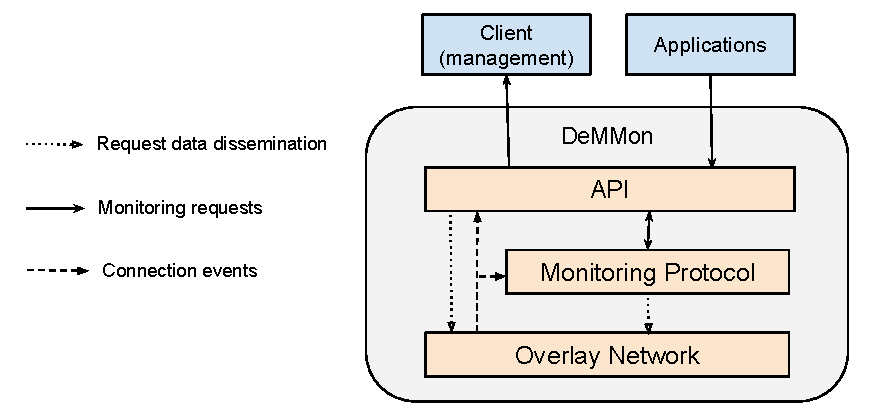
\includegraphics[width=\textwidth]{Chapters/Figures/DeMMon-arch-overview.pdf}
    \caption{An overview of the architecture of DeMMon}
    \label{fig:demmon-overview}
\end{figure}


\begin{enumerate}
    \item The overlay network, which strives to build the tree-shaped network, nodes in this network use proximity and a set of logical rules to change their location in the tree.

    \item The monitoring protocol, which is a component that collects and disseminates information using the overlay network's established connections. It communicates via notifications and asynchronous request-replies with the overlay network to receive updates regarding established connections and connection failures. Lastly, it receives requests from the API to collect information.

    \item Lastly, the API receives updates from both the overlay network and the monitoring protocol, exposes the received information from those layers, and allows ingestion of new information. Furthermore, it allows issuing commands to collect new information, perform local aggregations periodically, or trigger issued alarms based on the respective conditions.
\end{enumerate}

\section{Overlay network}

In this section, we discuss the design of the aforementioned distributed membership protocol, which aims at building and maintaining a latency and bandwidth aware tree-shaped overlay network. We begin by providing the considered system model, followed by an overview of both the mechanisms responsible for building and maintaining the tree and lastly conclude with a summary and discussion.

\subsection{System Model}



\subsection{Overview}

\subsection{Summary}

\section{Monitoring protocol}

\subsection{Overview}

\subsection{Aggregation mechanisms}

\subsubsection{Single root aggregation}

\subsubsection{Multi root aggregation}

\subsubsection{Neighborhood aggregation}

\subsection{Summary}

\section{API}

\subsection{System Model}

\subsection{Overview}

\subsection{Showcase}